\documentclass{beamer}

\usepackage{animate}
\usepackage{subfigure}
\usetheme{AnnArbor}
\usecolortheme{beaver}

\title 
{Clustering Astronomical Data}
\subtitle
{5 Clustering Methods Compared}
\author{Dane Skinner \and Nick Hockensmith \and Kevin Park}
\institute
{Oregon State University}
\date
{April 24, 2015}

\begin{document}
%----------------------------------
% FRAME 1: TITLE PAGE
%----------------------------------
\begin{frame}
 \titlepage
\end{frame}

%----------------------------------
% FRAME 2
%----------------------------------
\begin{frame}
\frametitle{Outline}
\begin{itemize}
\item Brief Introduction
\item Questions of Interest
\item Clustering Methods
\item Conclusion and Final Thoughts
\end{itemize}
\end{frame}
%----------------------------------
% FRAME 3
%----------------------------------
\begin{frame}
\frametitle{Introduction}
\begin{itemize}
\item We have about 1500 training observations and 50,000 test observations of variable star data.
\item The task is to cluster the data accurately.
\item We focus on the training data because it allows us to compare the known clusters to the clusters the algorithms assign to the observations.
\end{itemize}

\end{frame}

%----------------------------------
% FRAME 4
%----------------------------------

\begin{frame}
\frametitle{Questions of Interest}
\begin{itemize}
\item What clustering algorithms perform the best?
\item Does subsetting the data help (i.e. Does clustering in stages improve performance)?
\end{itemize}
\end{frame}

%----------------------------------
% FRAME 5
%----------------------------------

\begin{frame}
\frametitle{K-Means Clustering}
\begin{itemize}
\item Advantages: 
\begin{itemize}
\item Easy to implement. 
\item Built in function in R is relatively quick.
\end{itemize}
\item Disadvantages: 
\begin{itemize}
\item Poor performance when data has overlapping variable values.
\item NP-Hard problem.
\end{itemize}
\end{itemize}
\end{frame}

%----------------------------------------------------------------
% FRAME 5.5
%----------------------------------------------------------------

\begin{frame}
\frametitle{K-Means Clustering Results}
\begin{center}
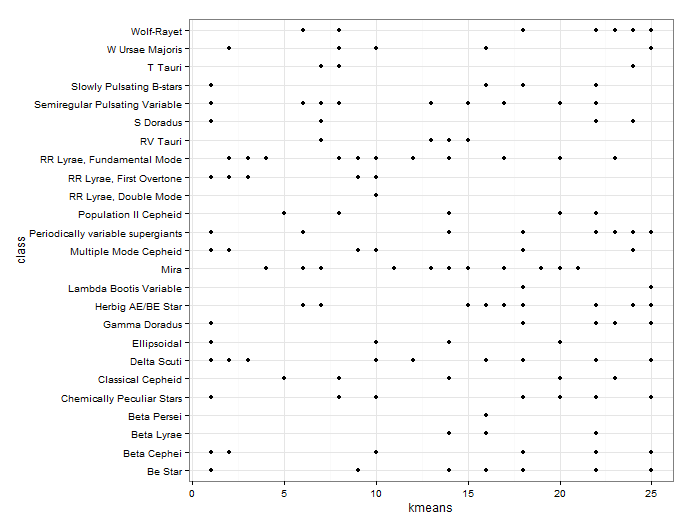
\includegraphics[scale=.4]{kmeans.png}
\end{center}
\end{frame}

%----------------------------------
% FRAME 6
%----------------------------------

\begin{frame}
\frametitle{K-Medoids Clustering}
\begin{itemize}
\item Advantages: 
\begin{itemize}
\item Improved performance over K-means.
\item Freedom to choose distance metric (typically any $\ell_p$ metric) although R only allows $\ell_1$ or $\ell _2$.
\end{itemize}
\item Disadvantages: 
\begin{itemize}
\item Performance still suffers when data has overlapping variable values.
\item Another NP-Hard problem.
\end{itemize}
\end{itemize}
\end{frame}

%----------------------------------------------------------------
% FRAME 6.5
%----------------------------------------------------------------

\begin{frame}
\frametitle{K-Medoids Clustering Results}
\begin{center}
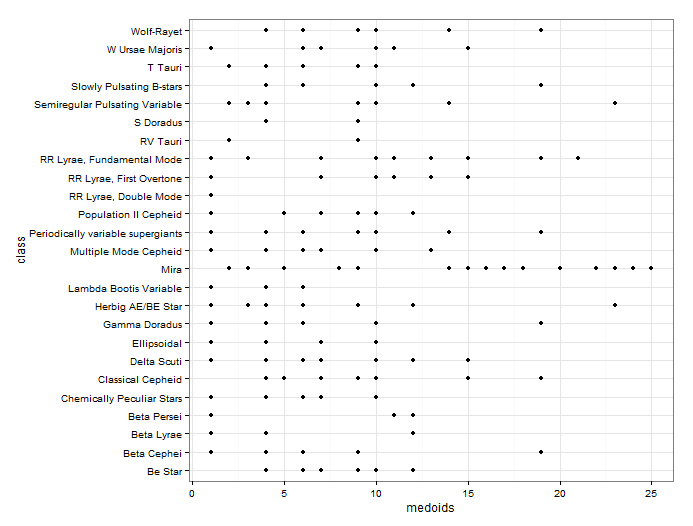
\includegraphics[scale=.4]{medoids.png}
\end{center}
\end{frame}
%----------------------------------
% FRAME 7
%----------------------------------
\begin{frame}
\frametitle{K-Means $++$}
\begin{itemize}
\item Advantages: 
\begin{itemize}
\item Iterative process yields improved performance over K-medoids.
\item Algorithm checks multiple possible cluster centers and returns best cluster assignments.
\end{itemize}
\item Disadvantages: 
\begin{itemize}
\item Iterative process takes time.
\item Algorithm may miss ideal solution since there are so many possible starting configurations.
\end{itemize}
\end{itemize}

\end{frame}

%----------------------------------------------------------------
% FRAME 8
%----------------------------------------------------------------

\begin{frame}
\frametitle{K-Means++ Clustering Results}
\begin{center}
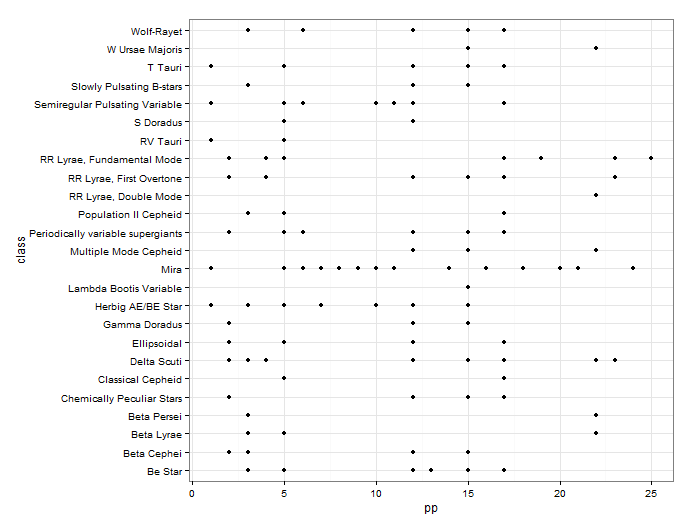
\includegraphics[scale=.4]{pp.png}
\end{center}
\end{frame}


%----------------------------------
% FRAME 9
%----------------------------------
\begin{frame}
	\frametitle{Spectral Clustering Methods}
		\begin{itemize}
			\item Chose the complete linkage over the single or average linkages
			\item All 85 explanatory variables were used for hierarchical clustering
			\item Each column variable was normalized to the interval $[0,1]$ via
				\begin{align*}
					x_i^{*} &= \frac{x_i-x_{min}}{x_{max}-x_{min}}
				\end{align*}
			\item Advantages:
			\begin{itemize}
				\item Adjusts column variables to a notionally common scale
				\item ``Better" spread in observation assignment to different clusters
				\item Quick run time
			\end{itemize}
			\item Disadvantages
			\begin{itemize}
				\item Algorithm still wants to push many observations into a small number of clusters
				\item Artificial scaling of units may or may not be a good thing
			\end{itemize}
		\end{itemize}
\end{frame}

%----------------------------------
% FRAME 10
%----------------------------------
\begin{frame}

	\frametitle{Tables}
\begin{table}[H]
\center
\begin{tabular}{c c c c c c c c c c c c c}
\hline
C. ID           & 1 & 2 & 3 & 4 & 5 & 6 & 7 & 8 & 9 & 10 & 11 & 12  \\
Obs. 		 &196 & 38 & 11 & 171 & 298 & 102 & 39 & 9 & 38 & 39 & 55 & 21  \\
\hline
C. ID           & 13 & 14 & 15 & 16 & 17 & 18 & 19 & 20 & 21 & 22 & 23 & 24  \\
Obs.         	& 1 & 13 & 11 & 17 & 3 & 6 & 11 & 4 & 4 & 1 & 3 & 6  \\
\hline
\end{tabular}
\caption{Farthest-Neighbor on Non-subsetted Training Data: Normalized (3)}
\begin{tabular}{c c c c c c c c c c c c c}
\hline
C. ID           & 1 & 2 & 3 & 4 & 5 & 6 & 7 & 8 & 9 & 10 & 11 & 12  \\
Obs. 		 & 856 & 22 & 7 & 4 & 37 & 81 & 4 & 11 & 45 & 1 & 2 & 1  \\
\hline
C. ID           & 13 & 14 & 15 & 16 & 17 & 18 & 19 & 20 & 21 & 22 & 23 & 24  \\
Obs.         	 & 6 & 2 & 12 & 7 & 2 & 1 & 1 & 1 & 1 & 1 & 1 & 3  \\
\hline
\end{tabular}
\caption{Farthest-Neighbor on Non-subsetted Training Data: Standardized (1)}
\end{table}
\end{frame}

%----------------------------------
% FRAME 11
%----------------------------------
\begin{frame}
	\frametitle{Dendrograms}
\begin{figure}[h]
	\begin{center}	
		\subfigure[All Star types ]{
		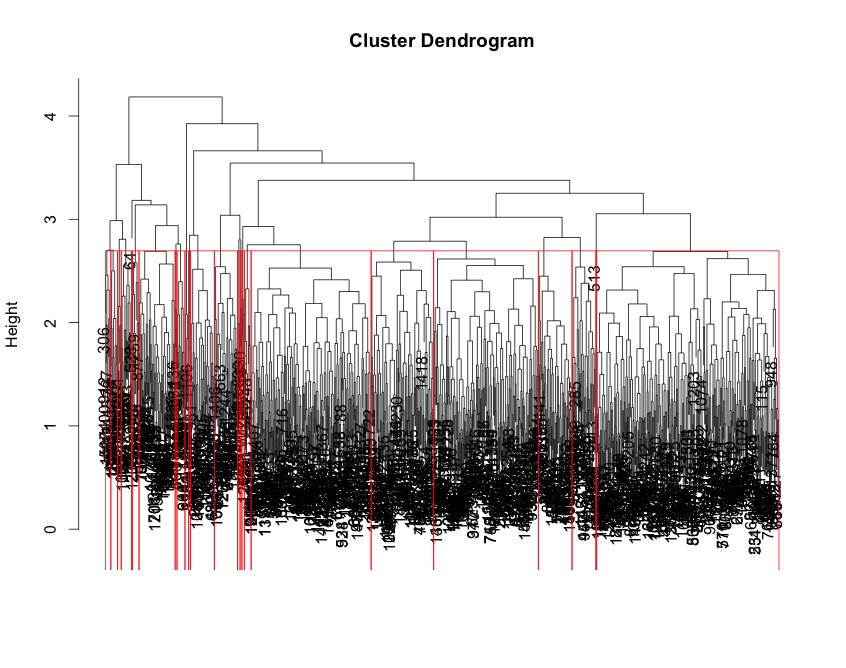
\includegraphics[scale=0.18]{dendro24group.jpeg}}
		\subfigure[Pulsating Star types only]{
		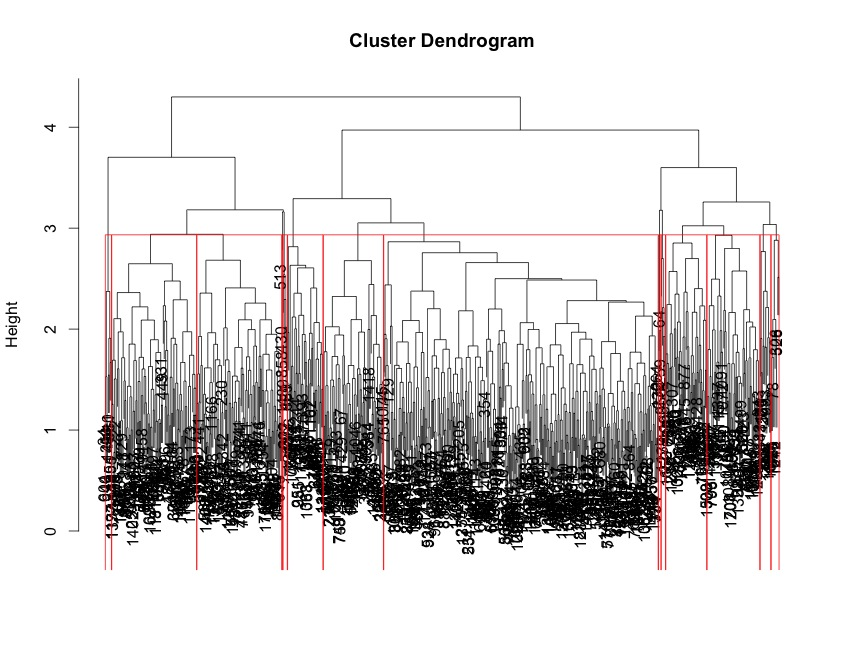
\includegraphics[scale=0.18]{dendro14group.jpeg}}
	\end{center}
\end{figure} 
\end{frame}

%----------------------------------
% FRAME 12
%----------------------------------
\begin{frame}
	\frametitle{Dendrograms}
\begin{figure}[h]
	\begin{center}	
		\subfigure[Eruptive Star types only]{
		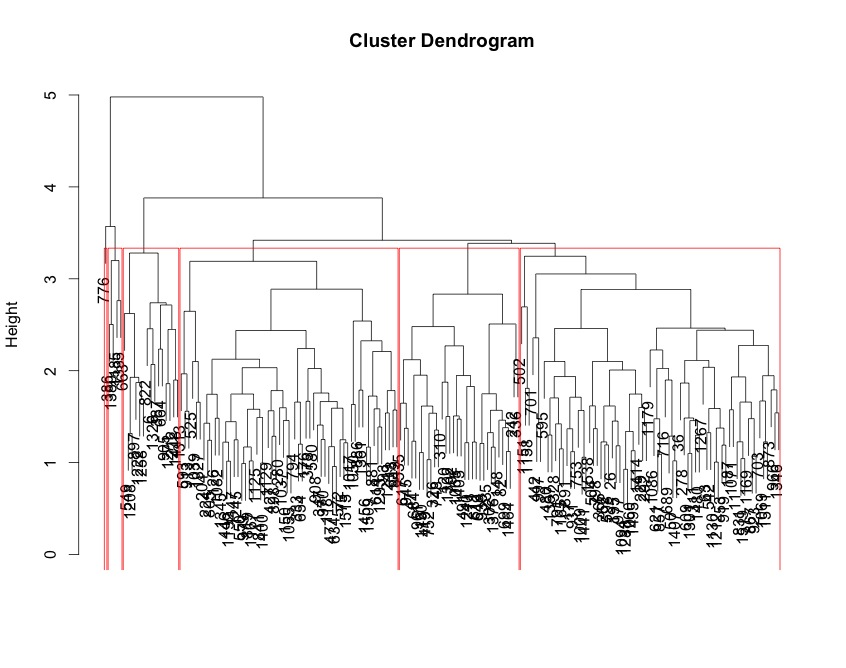
\includegraphics[scale=0.17]{dendro6group.jpeg}}
		\subfigure[Multi-Star types only]{
		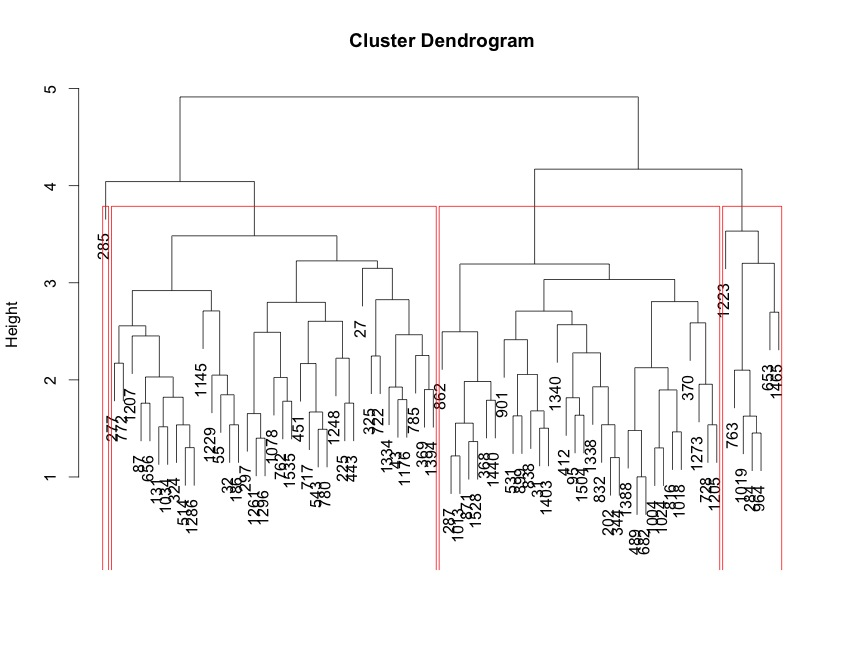
\includegraphics[scale=0.17]{dendro4group.jpeg}}
	\end{center}
\end{figure} 
\end{frame}

%----------------------------------
% FRAME 13
%----------------------------------
\begin{frame}
	\frametitle{Spectral Clustering Results}
\begin{figure}[h]
	\begin{center}	
		\subfigure[All Star types ]{
		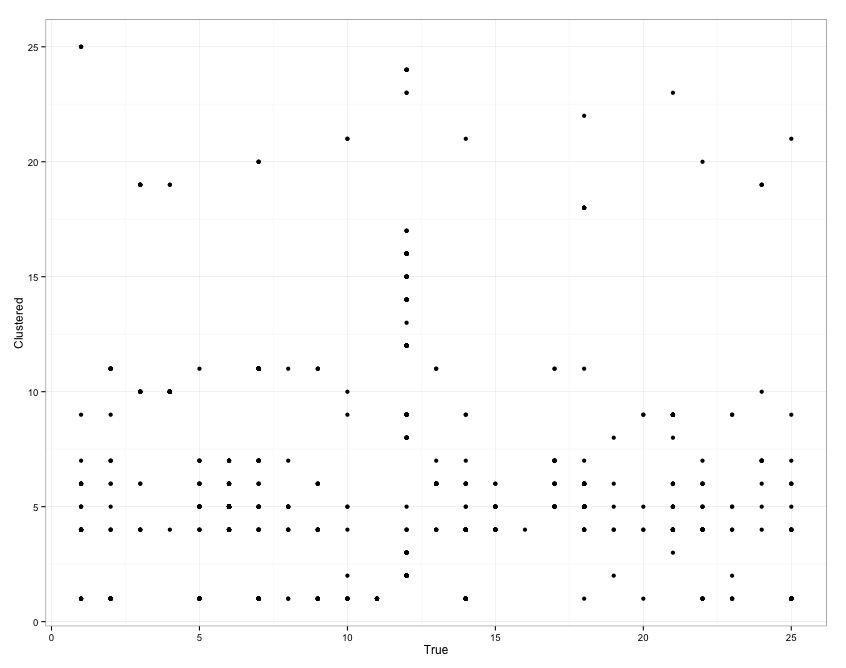
\includegraphics[scale=0.17]{TvCall25.jpeg}}
		\subfigure[Pulsating Star types only]{
		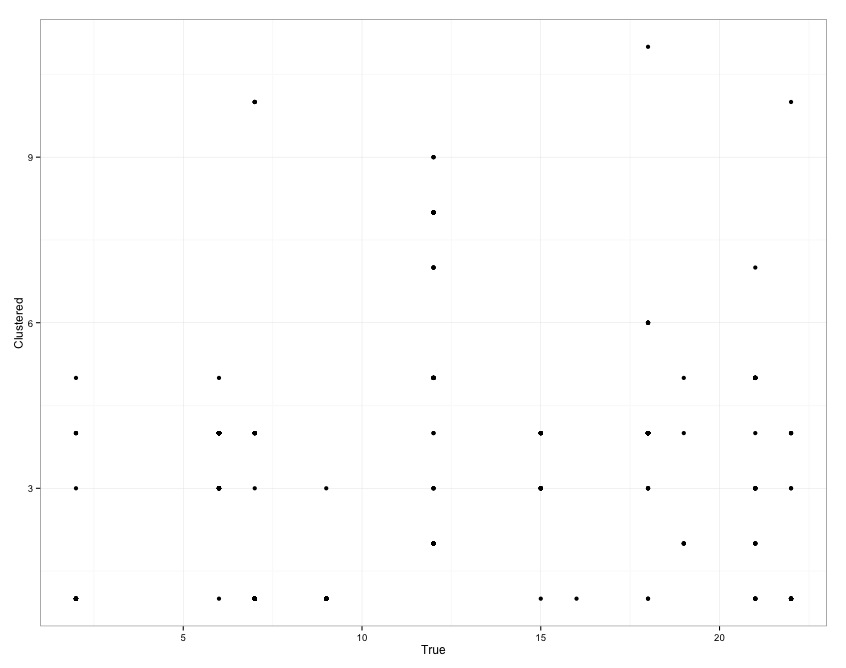
\includegraphics[scale=0.17]{TvCpulse11.jpeg}}
	\end{center}
\end{figure} 
\end{frame}

%----------------------------------
% FRAME 14
%----------------------------------

\begin{frame}
	\frametitle{Spectral Clustering Results}
\begin{figure}[h]
	\begin{center}	
		\subfigure[Eruptive Star types only]{
		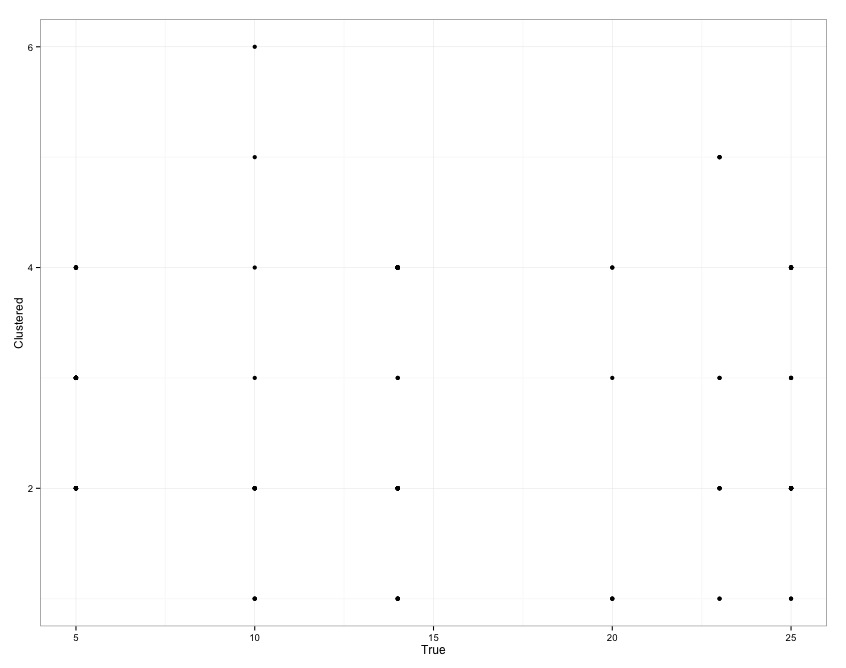
\includegraphics[scale=0.17]{TvCerupt.jpeg}}
		\subfigure[Multi-Star types only]{
		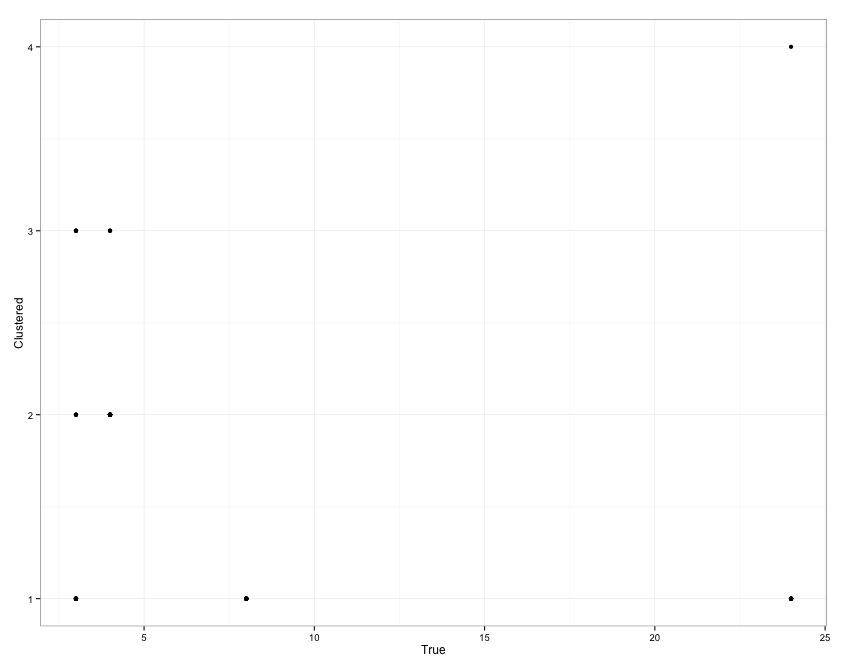
\includegraphics[scale=0.17]{TvCmulti.jpeg}}
	\end{center}
\end{figure} 
\end{frame}

%----------------------------------
% FRAME 15
%----------------------------------

\begin{frame}
	\frametitle{Conclusions and Final Thoughts}
\end{frame}
\end{document}
